\documentclass[../main.tex]{subfiles}

\begin{document}
\section{Chips Architecture}
The Chips architecture was designed with the intent of being able to mix and match chips. In order to mix and match chips, the sub-designs (ie. chips) need to be designed in a way that they can be connected through an interposer. This assembly structure is called 2.5D (Physical layer). Figure ?? shows relationship of the die to interposer connections. The SOC is designed to run over-top of AIB. The SOC contains three bus, two are configured as AXI and the other one is configured as CIPI. The SOC connects the ciplets together. There are two types of ciplets: controllers and accelerators.

\subsection{Physical Layer}
The Physical layer is made up of banks of AIB Drivers. The AIB Driver has the ability to send and receive data or clock. One driver is configured for transmit and the other is configured for receive. The AIB drivers are design work over an interposer. Forty-eight drives make up a AIB channel. Eight of drivrs make up the clock and the rest are configured for transmit or receive. The eight clocks divers are broken up into 4 sets of differential pairs. Two clock sets are configured to transmit a clock, and the other two are for receiving the forward clock. The forward clock is used for re-syncing data. Figure ?? shows the layout of a AIB channel in the Chips Architecture.

\subsection{CHIPS SOC}
The CHIPs SOC uses two protocols: AXI and CIPI. The AXI protocol allows for point to point memory transactions. There are two buses that uses AXI and one bus that uses CIPI. The AXI bus is used for the on-chip and chip to chip commutation. The CIPI bus is used for off-chip commutation. The CIPI bus grows the size of the addressable memory space that that the system can access. With a large address space, larger work loads can be ran. The AXI bus are named XBus and MBus. The MBus connect the global shared memory space for all the chips. The XBus connects all the chips together. Its purpose is used to configure and control the accelerators. Figure ?? show the layout of the buses.

\subsection{Chiplets}
The controllers chiplets use the Rocket Chip IP\cite{Asanović:EECS-2016-17}. In this layout, there are two different layouts for the Rocket Chip, one was wrapped with AIB and the other was not. The two accelerators chiplets are LSTM and SCNN. Figure ?? shows the layout of the tape-out. Each major Design is hi highlighted. 
\subsubsection{Rocket Core}
%\begin{figure}
%    \centering
%    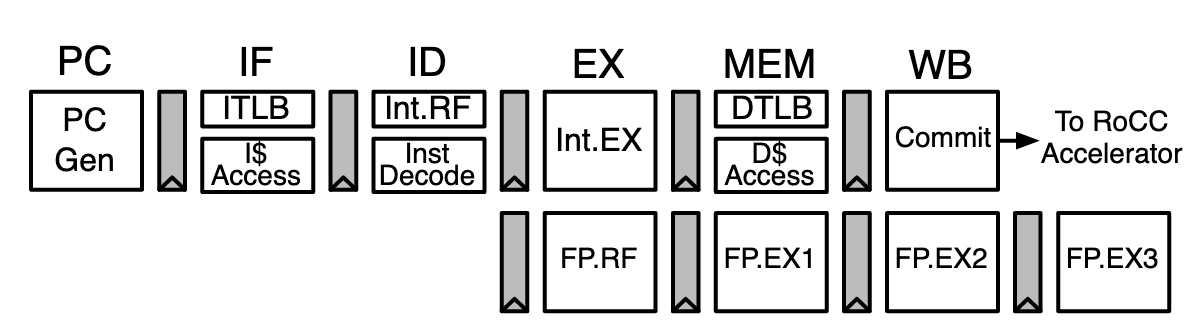
\includegraphics[scale=.4]{pngs/RocketPipeline.png}
%    \caption{Rocket Chkp Pipeline\cite{Asanović:EECS-2016-17}}
%    \label{fig:RocketChipPipeline}
%\end{figure}
The Rocket Core was generated by using the Rocket Chip Generator. The Rocket Chip Generator was developed by UC. Berkeley and is maintained by the CHIPS Alliance. Figure ?? shoe a high level overview of a default Rocket Chip. Starting form top to bottom: The Generator can be used to create N Number of Tiles. Tiles are the most basic 
\subsubsection{LSTM}
\blindtext
\subsubsection{SCNN}
\blindtext
\end{document}

